\documentclass[letterpaper,11pt, reqno]{amsart}

\usepackage{amsfonts, amsthm, amssymb, amsmath, stmaryrd}
\usepackage{bbm}
\usepackage{mathrsfs,array}
\usepackage{eucal,fullpage,times,color,enumerate,accents,mathtools}
\usepackage{url}
\usepackage{scalerel,stackengine}
\usepackage{dotlessj}
\usepackage{cancel}
\usepackage{pgfplots}
\usepackage{colortbl,hhline}
\usepackage{tikz}
\usetikzlibrary{decorations.pathmorphing}
\usetikzlibrary{patterns}
\usetikzlibrary{arrows}
\usepackage[all]{xy}
\usepackage{soul}
\usepackage{xcolor}
\usepackage{etoolbox}
\usepackage{pifont}
\usetikzlibrary{fadings}
\usetikzlibrary{calc}
\usepackage{listings}
\usepackage{wasysym}
\tikzfading[name=fade out,
  inner color=transparent!0, outer color=transparent!100]
\tikzfading[name=fade right,
  left color=transparent!0, right color=transparent!100]
\tikzfading[name=fade left,
  right color=transparent!0, left color=transparent!100]
\tikzfading[name=fade mid,
  left color = transparent!100, right color = transparent!100, middle color=transparent!0]
\usepackage{ifthen}
\tikzset{
  laser beam action/.style={
    line width=\pgflinewidth+1.4pt,draw opacity=.095,draw=#1,
  },
  laser beam recurs/.code 2 args={%
    \pgfmathtruncatemacro{\level}{#1-1}%
    \ifthenelse{\equal{\level}{0}}%
    {\tikzset{preaction={laser beam action=#2}}}%
    {\tikzset{preaction={laser beam action=#2,laser beam recurs={\level}{#2}}}}
  },
  laser beam/.style={preaction={laser beam recurs={20}{#1}},draw opacity=1,draw=#1},
}
\usepackage{graphics}
\usepackage{graphicx}
\usepackage[export]{adjustbox}
\usepackage[curve]{xypic}
\usepackage{bm}
\usetikzlibrary{calc}
\usepackage[font=small,labelfont=bf]{caption}
\usepackage{stackengine,scalerel,graphicx}
\savestack\UAtextstyle{\stackon[-2.7pt]{$\rule[2.3pt]{4pt}{.35pt}$}{\scalebox{-1}{$U$}}}
\def\UA{\scalerel*{\UAtextstyle}{X}}
\usepackage{arydshln}



\definecolor{navy}{rgb}{0,0,.65}

%This reverse-links the references in the paper. Useful for large papers.
\usepackage[colorlinks]{hyperref}
\hypersetup{colorlinks=true,urlcolor=teal,linkcolor=navy,citecolor=navy}

\makeatletter
\def\@tocline#1#2#3#4#5#6#7{\relax
  \ifnum #1>\c@tocdepth % then omit
  \else
    \par \addpenalty\@secpenalty\addvspace{#2}%
    \begingroup \hyphenpenalty\@M
    \@ifempty{#4}{%
      \@tempdima\csname r@tocindent\number#1\endcsname\relax
    }{%
      \@tempdima#4\relax
    }%
    \parindent\z@ \leftskip#3\relax \advance\leftskip\@tempdima\relax
    \rightskip\@pnumwidth plus4em \parfillskip-\@pnumwidth
    #5\leavevmode\hskip-\@tempdima
      \ifcase #1
       \or\or \hskip 1em \or \hskip 2em \else \hskip 3em \fi%
      #6\nobreak\relax
    \dotfill\hbox to\@pnumwidth{\@tocpagenum{#7}}\par
    \nobreak
    \endgroup
  \fi}
\makeatother

\renewcommand{\familydefault}{ppl}
\setlength{\marginparwidth}{1in}
\setlength{\marginparsep}{0in}
\setlength{\marginparpush}{0.1in}
\setlength{\topmargin}{0in}
\setlength{\headheight}{0pt}
\setlength{\headsep}{0pt}
\setlength{\footskip}{.3in}
\setlength{\textheight}{9.0in}
\setlength{\textwidth}{6.25in}
\setlength{\parskip}{0pt}

%\newtheorem{theorem}{Theorem}[section]
\newtheorem{idea}{Musical proto-idea}[]
\renewcommand*{\theidea}{\arabic{idea}}
\newtheorem{ideaB}{Simple musical idea}[]
\renewcommand*{\theideaB}{\arabic{ideaB}}
\newtheorem{composition}{Composition}[]
\renewcommand*{\thecomposition}{\Alph{composition}}
\newtheorem{theorem}{Theorem}[subsection]
\newtheorem{monodromy theorem}{Monodromy Theorem}[subsection]
\newtheorem{corollary}[theorem]{Corollary}
\newtheorem{hypothesis}[theorem]{Hypothesis}
\newtheorem{wild conjecture}[theorem]{Wild Conjecture}
\newtheorem{claim}[theorem]{Claim}
\newtheorem{lemma}[theorem]{Lemma}
\newtheorem{proposition}[theorem]{Proposition}
\newtheorem{definition}[theorem]{Definition}
\newtheorem{warning}[theorem]{Warning}
\newtheorem{research objectives}{Research objectives}[subsection]
\newtheorem{questions}{Question}
\newtheorem{question}[theorem]{Question}
\newtheorem{research question}[theorem]{Research questions}
\newtheorem{answer}[theorem]{Answer}
\newtheorem{aside question}[theorem]{Aside question}
\newtheorem{exercise}[theorem]{Exercise}
\newtheorem{sketch}[theorem]{Sketch}
\newtheorem{aside}[theorem]{Aside}
\newtheorem{problem}[theorem]{Problem}
\newtheorem{conjecture}[theorem]{Conjecture}
\newtheorem{assumption}[theorem]{Assumption}
\newtheorem{construction}[theorem]{Construction}
\newtheorem{example}[theorem]{Example}
\newtheorem{examples}[theorem]{Examples}
\newtheorem{audio example}[theorem]{\loudspeaker[3] Example}
\newtheorem{quasi-theorem}[theorem]{Quasi-Theorem}
\newtheorem{prop/def}[theorem]{Proposition/Definition}
\newtheorem{blank remark}[theorem]{}
\newtheorem{ssubsection}[theorem]{}
\newtheorem{terminology and comment}[theorem]{Terminology and comment}
\newtheorem{fact}[theorem]{Fact}
\newtheorem{computation}[theorem]{Computation}
\newtheorem{observation}[theorem]{Observation}
\newtheorem{algorithm}[theorem]{Algorithm}
\newtheorem{setup}[theorem]{Setup}
\newtheorem{purity hypothesis}[theorem]{Purity hypothesis}
\newtheorem{corollary of the purity hypothesis}[theorem]{Corollary of the purity hypothesis}

%Theorem indexed with letters A, B, C, ...
\newtheorem{Th}{Theorem}[]
\renewcommand*{\theTh}{\Alph{Th}}

\newtheorem{rem1}[theorem]{Remark}
\newenvironment{remark}{\begin{rem1}\em}{\end{rem1}}

\newtheorem{not1}[theorem]{Notation}
\newenvironment{notation}{\begin{not1}\em}{\end{not1}}

%% Math Blackboard
\newcommand{\A}{{\mathbb{A}}}           
\newcommand{\CC} {{\mathbb C}}       
\newcommand{\DD} {{\mathbb D}}
\newcommand{\EE}{\mathbb{E}}
\newcommand{\GG}{\mathbb{G}}
\newcommand{\LL}{\mathbb{L}}
\newcommand{\NN} {{\mathbb N}}		
\newcommand{\PP}{\mathbb{P}}         
\newcommand{\QQ} {{\mathbb Q}}		
\newcommand{\RR} {{\mathbb R}}		
\newcommand{\Circ} {{\mathbb S}}		
\newcommand{\ZZ} {{\mathbb Z}}		
\newcommand{\TT} {{\mathbb T}}	
\newcommand{\FF}{{\mathbb F}}

%%Presuperscript
\def\presuper#1#2%
  {\mathop{}%
   \mathopen{\vphantom{#2}}^{#1}%
   \kern-\scriptspace%
   #2}
	
\newcommand{\BC}{\text{BC}}

\DeclareMathOperator{\Aut}{Aut}
\DeclareMathOperator{\Gal}{Gal}
\DeclareMathOperator{\Circpec}{Spec_{\ \!}}
\DeclareMathOperator{\Split}{split}
\DeclareMathOperator{\Div}{div}
\DeclareMathOperator{\ord}{ord_{\ \!}}

\newcommand{\model}[1]{{\slantbox[.5]{$\mathcal{#1}$}\ }}

\newcommand{\lra}{{\longrightarrow}}
\DeclareMathOperator{\Def}{\overset{{}_{\text{def}}}{=}}

% slant box
\newsavebox{\foobox}
\newcommand{\slantbox}[2][.5]
  {%
    \mbox
      {%
        \sbox{\foobox}{#2}%
        \hskip\wd\foobox
        \pdfsave
        \pdfsetmatrix{1 0 #1 1}%
        \llap{\usebox{\foobox}}%
        \pdfrestore
      }%
  }

%%Prettier monomorphism and epimorphism arrows
\newcommand{\mono}{\!\xymatrix{{}\ar@{^{(}->}[r]&{}}\!}
\newcommand{\epi}{\!\xymatrix{{}\ar@{->>}[r]&{}}\!}
\newcommand{\rat}{\!\xymatrix{{}\ar@{-->}[r]&{}}\!}

%%Young diagram
\newcommand{\young}{\scalebox{.7}{$\pmb{\square\!\square}${\larger\larger $\pmb{\cdot\!\cdot\!\cdot}$}$\pmb{\square}$}}

%smaller subscript closed field
\newcommand{\lilF}{\mbox{{\smaller\smaller\smaller\smaller\smaller $\overline{\FF_{\!q}}$}}}

\newcommand{\iso}{\cong}
\newcommand{\disc}{\text{disc}}

% Tyler comments
\newcommand{\tyler}[1]{{\color{red} [#1\ \ \textemdash Tyler]}}

% Some slanted letters
\newcommand{\TP}{\slantbox[.3]{$\mathcal{TP}$}}

%Left action
\newcommand{\lact}{\ \raisebox{8pt}{\rotatebox{-90}{$\circlearrowright$}}\ }

%Left quotient
\newcommand{\lquot}[2]{\raisebox{-1.5pt}{$#1$}\big\backslash\raisebox{1.5pt}{$#2$}}

%Right quotient
\newcommand{\rquot}[2]{\raisebox{1.5pt}{$#1$}/\raisebox{-1.5pt}{$#2$}}

%importantmatrix
\newcommand{\MM}{\big(\begin{smallmatrix}0 & -1\\ 1 & -1\end{smallmatrix}\big)}

%compactified spec
\newcommand{\SpecZN}[1]{\overline{\text{Spec}_{\ \!}\ZZ}{}^{(#1)}}
\newcommand{\SpecZ}{\overline{\text{Spec}_{\ \!}\ZZ}}

%nice sep
\newcommand{\sep}{\textsf{sep}}

%nice res
\newcommand{\res}{\text{res}^{\eta}_{s}}

%nice sp
\newcommand{\spe}{\bold{Sp}}

%nice Sh
\newcommand{\Sh}{\bold{Sh}}

%nice et
\newcommand{\et}{\text{\'et}}

%nice M_g bar
\newcommand{\Mg}{{\ \ \overline{\!\!\mathscr{M}_{g}}}}
\newcommand{\Mgmbar}{\overline{M_{g}{\!\!}^{\text{{\smaller\smaller\smaller\smaller\smaller $\ (m)$}}}}}
\newcommand{\Mgm}{M_{g}{\!\!}^{\text{{\smaller\smaller\smaller\smaller\smaller $\ (m)$}}}}


\stackMath
\newcommand\reallywidehat[1]{%
\savestack{\tmpbox}{\stretchto{%
  \scaleto{%
    \scalerel*[\widthof{\ensuremath{#1}}]{\kern-.6pt\bigwedge\kern-.6pt}%
    {\rule[-\textheight/2]{1ex}{\textheight}}%WIDTH-LIMITED BIG WEDGE
  }{\textheight}% 
}{0.5ex}}%
\stackon[1pt]{#1}{\tmpbox}%
}

%changed footnote style
\renewcommand{\thefootnote}{[\arabic{footnote}]}

\numberwithin{equation}{theorem}

%
\newcounter{totfigures}

\providecommand\totfig{} 

\makeatletter
\AtEndDocument{%
  \addtocounter{totfigures}{\value{figure}}%
  \immediate\write\@mainaux{%
    \string\gdef\string\totfig{\number\value{totfigures}}%
  }%
}
\makeatother

\pretocmd{\chapter}{\addtocounter{totfigures}{\value{figure}}\setcounter{figure}{0}}{}{}


\newcommand{\midarrow}{\tikz \draw[-triangle 90] (0,0) -- +(.1,0);}



\usepackage{epigraph}
\setlength\epigraphwidth{.8\textwidth}
\setlength\epigraphrule{0pt}




\definecolor{codegreen}{rgb}{0,0.6,0}
\definecolor{codegray}{rgb}{0.5,0.5,0.5}
\definecolor{codepurple}{rgb}{0.58,0,0.82}
\definecolor{backcolour}{rgb}{0.95,0.95,0.92}

\lstdefinestyle{mystyle}{
    backgroundcolor=\color{backcolour},   
    commentstyle=\color{codegreen},
    keywordstyle=\color{magenta},
    numberstyle=\tiny\color{codegray},
    stringstyle=\color{codepurple},
    basicstyle=\ttfamily\footnotesize,
    breakatwhitespace=false,         
    breaklines=true,                 
    captionpos=b,                    
    keepspaces=true,                 
    numbers=left,                    
    numbersep=5pt,                  
    showspaces=false,                
    showstringspaces=false,
    showtabs=false,                  
    tabsize=2
}

\lstset{style=mystyle}





\newcommand{\ExternalLink}{%
    \tikz[x=1.2ex, y=1.2ex, baseline=-0.05ex]{% 
        \begin{scope}[x=1ex, y=1ex]
            \clip (-0.1,-0.1) 
                --++ (-0, 1.2) 
                --++ (0.6, 0) 
                --++ (0, -0.6) 
                --++ (0.6, 0) 
                --++ (0, -1);
            \path[draw, 
                line width = 0.5, 
                rounded corners=0.5] 
                (0,0) rectangle (1,1);
        \end{scope}
        \path[draw, line width = 0.5] (0.5, 0.5) 
            -- (1, 1);
        \path[draw, line width = 0.5] (0.6, 1) 
            -- (1, 1) -- (1, 0.6);
        }
    }


\usepackage{caption}
\captionsetup{font=footnotesize}

\usepackage{graphicx}
\newcommand\vcent[1]{\vcenter{\hbox{#1}}}
\newcommand\loudspeaker[1][3]{\ensuremath{\vcent{\rule{.6ex}{.6ex}}\kern-.5ex%
  \vcent{\scalebox{.6}[1]{\rotatebox[origin=center]{90}{$\blacktriangle$}}}%
  \ifnum#1>0\relax\kern.1ex\vcent{\scalebox{.4}{)}}\ifnum#1>1\relax\kern-.1ex%
  \vcent{\scalebox{.55}{)}}\ifnum#1>2\relax\kern-.15ex\vcent{\scalebox{.7}{)}}%
  \fi\fi\fi}%
}



\newcommand\modulo[2]{\@tempcnta=#1
        \divide\@tempcnta by #2
        \multiply\@tempcnta by #2
        \multiply\@tempcnta by -1
        \advance\@tempcnta by #1\relax
        \the\@tempcnta}
\makeatother


\makeatletter
\newcommand*{\doublerightarrow}[2]{\mathrel{
  \settowidth{\@tempdima}{$\scriptstyle#1$}
  \settowidth{\@tempdimb}{$\scriptstyle#2$}
  \ifdim\@tempdimb>\@tempdima \@tempdima=\@tempdimb\fi
  \mathop{\vcenter{
    \offinterlineskip\ialign{\hbox to\dimexpr\@tempdima+1em{##}\cr
    \rightarrowfill\cr\noalign{\kern.5ex}
    \rightarrowfill\cr}}}\limits^{\!#1}_{\!#2}}}
\newcommand*{\triplerightarrow}[1]{\mathrel{
  \settowidth{\@tempdima}{$\scriptstyle#1$}
  \mathop{\vcenter{
    \offinterlineskip\ialign{\hbox to\dimexpr\@tempdima+1em{##}\cr
    \rightarrowfill\cr\noalign{\kern.5ex}
    \rightarrowfill\cr\noalign{\kern.5ex}
    \rightarrowfill\cr}}}\limits^{\!#1}}}
\makeatother




%%%%%%%%%%%%%%%%%%%%%%%%%%%%%%%%%%%%%%
%%%%%%%%%%%%%%%%%%%%%%%%%%%%%%%%%%%%%%

\setcounter{tocdepth}{2}


\title{{\smaller\smaller\smaller\smaller\it Notes on}\\ \ \\ Tonal Theories\\ {\smaller\smaller\smaller\it coming from} Representations of\\ Algebraic Groups {\smaller\smaller\smaller\it other than} $\text{GL}_{\pmb{1}}\pmb{(\CC)}$\\ \ \\ \ {\smaller\smaller\smaller\smaller\it \textemdash\ In progess\ \textemdash}}
\date{\today}
\author{Tyler Foster}

\begin{document}

\maketitle

\begin{abstract}
   Lots of the structure of tonal harmony emerges from the representation theory of $\text{GL}_{1}(\CC)$. I here begin the project of composing music using tonal structures that emerge from the representation theory of other, higher-dimensional algebraic groups, such as $\text{SL}_{2}(\CC)$. This isn't just some theoretical exercise. As these notes should make clear, implementing these tonal structures in code will be very difficult to pull off without the super detailed outline of the general theory that appears below.
\end{abstract}

\tableofcontents

\begin{section}{Homogeneous polynomials and chords.}

\begin{subsection}{Decomposing complex numbers for better signal analysis}
Fix an element $z\in\CC$. Fixing a positive real {\em period} $P\in\RR_{>0}$ once and for all, we can decompose $z$ into its real and imaginary parts as
	\begin{equation}\label{complex decomp}
	z
	\ =\ 
	z(A,\theta)
	\ =\ 
	\text{log}(A)+i\tfrac{2\pi}{P}\theta,
	\end{equation}
for unique $0<A<\infty$ and $0\le \theta<P$. We refer to the positive real number $$\lambda:=\frac{1}{P}$$ as the {\em frequency} of $z(A,\theta)$. One reason for decomposing $z$ as in Equation \eqref{complex decomp} is that it gives the exponential of $z$ a form relevant to music. Indeed, from Equation \eqref{complex decomp} we get
	$$
	e^{z}
	\ =\ 
	A\ \!e^{i2\pi\lambda\theta},
	$$
with real and imaginary parts
	$$
	\text{Re}(e^{z})
	\ =\ 
	A\ \text{cos}(2\pi\lambda\theta)
	\ \ \ \ \ \ \ \ \ \text{and}\ \ \ \ \ \ \ \ \ 
	\text{Im}(e^{z})\ =\ A\ \text{sin}(2\pi\lambda\theta),
	$$
respectively. If we fix $A$ and let $\theta$ change linearly at the rate of $1$ unit per second, then both $\text{Re}(e^{z})$ and $\text{Im}(e^{z})$ describe a ``pure'' tone playing with amplitude $A$ at $\lambda\ \text{Hz}$,\footnote{\ Here $A$ is measured in units of $A_0 \ e^{20\text{dB}}$, where $A_{0}$ is some fixed reference amplitude.} such that the tone associated to $\text{Re}(e^{z})$ and the tone associated to $\text{Im}(e^{z})$ are out of phase by a quarter period $\frac{P}{4}$.

\end{subsection}

\begin{subsection}{Independent complex variables}
Suppose now that we choose two complex numbers $z_1,z_2\in\CC$, independently of one another, with corresponding exponentials
	\begin{equation}\label{same P}
	e^{z_1}
	=
	A_1\ e^{i2\pi\lambda\theta_1}
	\ \ \ \ \ \ \ \ \ \ \text{and}\ \ \ \ \ \ \ \ \ 
	e^{z_2}
	=
	A_2\ e^{i2\pi\lambda\theta_2}.
	\end{equation}
In Equation \eqref{same P}, we assume that we've fixed a single period $P$, hence a single frequency $\lambda$, that $z_1$ and $z_2$ share. However, we could just as well choose two different periods, $P_1$ and $P_2$ say, and thus two different frequencies $\lambda_1=\tfrac{1}{P_1}$ and $\lambda_2=\tfrac{1}{P_2}$, to get
	$$
	e^{z_1}
	=
	A_1\ e^{i\tfrac{2\pi}{P_1}\theta_1}
	=
	A_1\ e^{i2\pi\lambda_1\theta_1}
	\ \ \ \ \ \ \ \ \ \ \text{and}\ \ \ \ \ \ \ \ \ 
	e^{z_2}
	=
	A_2\ e^{i\tfrac{2\pi}{P_2}\theta_2}
	=
	A_2\ e^{i2\pi\lambda_2\theta_2},
	$$
where $\lambda_1=\tfrac{1}{P_1}$ and $\lambda_2=\tfrac{1}{P_2}$. 

Given a function $f(x,y)$ of two variables, we can evaluate $f$ at $x=e^{z_1}$ and $y=e^{z_2}$ to obtain the value $f(e^{z_1},e^{z_2})$. In the special case that $f(x,y)$ is a {\em Laurent monomial}, i.e., that
	$$
	f(x,y)=x^my^n,
	$$
for $m,n\in\ZZ$, we have
	$$
	f(e^{z_1}, e^{z_2})
	\ =\ 
	A_1A_2\ e^{i2\pi (m\lambda_1\theta_1+n\lambda_2\theta_2)}
	\ =\ 
	A_1A_2\ e^{i2\pi\big(\tfrac{m}{P_1}\theta_1+\tfrac{n}{P_2}\theta_2\big)}.
	$$
The real and imaginary parts of this are
	\begin{equation}\label{FM style 1}
	\text{Re}\ f(e^{z_1}, e^{z_2})
	\ =\ 
	A_1A_2\ \text{cos}\Big(2\pi\big(\tfrac{m}{P_1}\theta_1+\tfrac{m}{P_2}\theta_2\big)\Big)
	\end{equation}
	$$
	\ \ \ \ \ \ \text{and}\ \ \ \ \ \ 
	$$
	\begin{equation}\label{FM style 2}
	\text{Im}\ f(e^{z_1}, e^{z_2})
	\ =\ 
	A_1A_2\ \text{sin}\Big(2\pi\big(\tfrac{m}{P_1}\theta_1+\tfrac{m}{P_2}\theta_2\big)\Big)
	.
	\end{equation}
This is a situation ripe for techniques from frequency modulation. For instance, if we let $t$ denote our time variable, in units of seconds, and we define
	$$
	\theta_1(t)\ =\ t
	\ \ \ \ \ \ \ \ \ \text{and}\ \ \ \ \ \ \ \ \ 
	\theta_2(t)\ =\ \text{sin}(\omega\ t)\ \ \ \text{for some}\ \omega\in\RR_{>0},
	$$
then the formulas in Equations \eqref{FM style 1} and \eqref{FM style 2} become instances of \href{https://en.wikipedia.org/wiki/Frequency_modulation_synthesis}{{\em FM synthesis}}. We can also see that the formulas in Equations \eqref{FM style 1} and \eqref{FM style 2} give us a broad generalization of FM synthesis, in that we can use any pair of real-valued functions
	$$
	\theta_1(t)\ \ \ \ \ \ \text{and}\ \ \ \ \ \ \ \theta_2(t)
	$$
of $t$ that we like. In this way, a kind of generalized FM synthesis realizes one version of the notion of ``pitch movement in $2$ dimensions.'' See Figure \ref{figure: ring modulation 2 dimensions}.
%It is important to keep in mind that the linear independence between the $2$ dimensions here is happening in the logarithm. In other words, the linear independence is in the variable $z$, not in the value $e^{z}$.
	\begin{figure}[ht]
	$$
	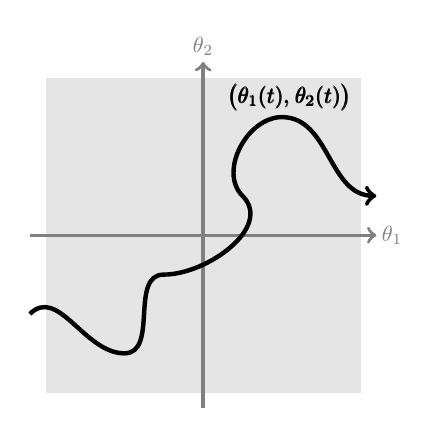
\begin{tikzpicture}
	\fill[black!10] (2,2) -- (-2,2) -- (-2, -2) -- (2, -2) -- cycle;
	\draw[black!50, very thick, ->] (-2.2,0) -- (2.2,0);
	\draw[black!50, very thick, ->] (0,-2.2) -- (0,2.2);
	\draw[black, ultra thick, ->] (-2.2,-1) to [out=45, in=180] (-1,-1.5) to [out=0, in=180] (-.5,-.5) to [out=0, in=-45] (.5,.5) to [out=135, in=180] (1, 1.5) to [out=0, in=180] (2.2,.5);
	\node[black!50] at (2.4, 0) {\scalebox{.8}{$\theta_1$}};
	\node[black!50] at (0, 2.4) {\scalebox{.8}{$\theta_2$}};	
	\node[black] at (1.1, 1.75) {\scalebox{.8}{$\pmb{\big(\theta_1(t),\ \!\theta_2(t)\big)}$}};
	\end{tikzpicture}
	$$
	\caption{General FM-synthesis from curves in the real plane.}
	\label{figure: ring modulation 2 dimensions}
	\end{figure}

%This begins to move into the realm of harmony. We pause our development of harmony here, and pick it back up in {\color{red} \S[...]}

\begin{example}
\normalfont
{\bf Ring modulation as a special case.}
Let us briefly remark here that, although it is not usually presented in this way, {\em ring modulation} in signal processing arises when we evaluate the real and imaginary parts of the monomial $xy$ at $x=e^{z_1}$ and $y=e^{z_2}$. In this way, ring modulation becomes a special case of the above discussion.
\end{example}

\end{subsection}

\begin{subsection}{Homogenous linear combinations of independent complex variables}
If $x$ and $y$ are independent complex variables, then a $\CC$-linear combination of monomials in $x$ and $y$, say
	\begin{equation}\label{homogeneous linear comb 1}
	a_{1}x^{m_1}y^{n_1}
	+
	a_{2}x^{m_2}y^{n_2}
	+
	\cdots
	+
	a_{\ell}x^{m_\ell}y^{n_\ell},
	\ \ \ a_1,a_2,\dots,a_\ell\in\CC
	\end{equation}
is {\em homogeneous of degree $d$} if $m_i+n_i=d$ for all $1\le i\le \ell$, in other words, if all monomials $x^my^n$ in the linear combination have the same {\em total degree} $m+n$, equal to $d$. When the linear combination in Equation \eqref{homogeneous linear comb 1} is homogeneous of degree $d$, we refer to it as a {\em homogeneous polynomial of degree $d$} in the variables $x$ and $y$ over $\CC$.

Notice that, from a musical perspective, a homogeneous linear combination in Equation \eqref{homogeneous linear comb 1} combines two distinct ideas in a way that isn't possible with a single variable. It packages multiple instances of ring modulation into a single chord-like structure. Indeed, 

The general homogeneous polynomial of degree $d$ in $x$ and $y$ can be written
	$$
	f(x,y)
	\ =\ 
	a_{0}x^d+a_1x^{d-1}y+a_2x^{d-2}y^2+\cdots+a_{d-1}xy^{d-1}+a_{d}y^d,
	$$
with coefficients $a_0,a_1,\dots,a_d\in\CC$. We can write this more succinctly as
	$$
	f(x,y)
	\ =\ 
	\sum_{n=0}^{d}a_nx^{d-n}y^n.
	$$
Evaluating this polynomial at $x=e^{z_1}$ and $y=e^{z_2}$, we obtain
	\begin{equation}\label{equation: homogeneous eval at e^z}
	f(e^{z_1},e^{z_2})
	\ =\ 
	\sum_{n=0}^{d}a_{n}A_{1}^{d-n}A_{2}^{n}e^{i2\pi\big(\tfrac{d-n}{P_1}\theta_1+\tfrac{n}{P_2}\theta_2\big)}.
	\end{equation}
To get a slightly clearer picture of this, let us assume that $a_i=1$ for all $0\le i\le d$ and that $A_1=A_2=1$. Then the right-hand side of Equation \eqref{equation: homogeneous eval at e^z} becomes
	\begin{equation}\label{equation: all amplitudes =1}
	\sum_{n=0}^{d}e^{i2\pi\big(\tfrac{d-n}{P_1}\theta_1+\tfrac{n}{P_2}\theta_2\big)}.
	\end{equation}
We play with this expression a bit more in Example \ref{example: relationship to standard chords} below.

\begin{example}\label{example: relationship to standard chords}
\normalfont
[...]

{\bf Special case: $\pmb{\theta_1=\theta_2}$ and $\pmb{P_1=P_2}$.}
	[...]
	Equation \eqref{equation: all amplitudes =1} becomes
	$$
	(d+1)e^{i2\pi\tfrac{d}{P}\theta}
	\ =\ 
	(d+1)e^{i2\pi d\lambda\theta}
	$$

{\bf Special case: $\pmb{\theta_1=0}$.}
	[...]
	Equation \eqref{equation: all amplitudes =1} becomes
	$$
	\sum_{n=0}^{d}e^{i2\pi\tfrac{n}{P}\theta}
	\ =\ 
	1
	+
	e^{i2\pi\tfrac{1}{P}\theta}
	+
	e^{i2\pi\tfrac{2}{P}\theta}
	+
	\dots
	+
	e^{i2\pi\tfrac{d}{P}\theta},
	$$
or in terms of frequency,
	$$
	1
	+
	e^{i2\pi \lambda\theta}
	+
	e^{i2\pi 2\lambda\theta}
	+
	\dots
	+
	e^{i2\pi d \lambda\theta}.
	$$
Ignoring the constant term ``$1$,'' this is just an equi-voiced\footnote{\ We say that a chord is {\em equi-voiced} if the notes of a chord are equally loud. I don't know if this is standard terminology.} overtone chord with root at $\lambda\ \text{Hz}$.
\end{example}

\begin{question}
\normalfont
{\color{red} [Voicing and orchestration questions...]}
\end{question}


\begin{remark}
\normalfont
{\color{red} [Model movement of several $(\theta_1,\ \theta_2)$-pairs on particle dynamics in $2$-dimensional space. This provides an FM version of the particle dynamics experiment from {\em Voice Leader\ \textemdash\ DISPL.}...]}
\end{remark}
[...]
\end{subsection}



\end{section}

\vskip 1cm

\begin{section}{Representations of $\text{SL}_{2}(\CC)$.}

We let $\text{SL}_{2}(\CC)$ act on $\CC[x,y]$ through its inverse action on the argument $(x,y)$ of each function $f(x,y)\in\CC[x,y]$. Thus the matrix $\left(\begin{smallmatrix}a & b\\ c & d\end{smallmatrix}\right)\in\text{SL}_{2}(\CC)$ acts on each $f(x,y)\in\CC[x,y]$ via the action of its inverse $\left(\begin{smallmatrix}d & -b\ \\ -c\  & a\end{smallmatrix}\right)$

\end{section}


	







\vskip .75cm

\end{document}
